\section{Implementation}
The Laplace approximation has been implemented in \verb|Pytorch| \cite{pytorch2} using Generalized Gauss-Newton approximation for convex loss functions to guarantee that $\Sigma_{\theta^\ast}$ is positive semidefinite, as discussed in \cite{dauphin2024neglectedhessiancomponentexplains, ksnxr_ggn}.  The example with the banana distribution has been implemented with a loss that is linear in the model parameters, and therefore uses the exact Hessian.

The Bayesian quadrature model is implemented with \verb|emukit| \cite{emukit2019, emukit2023}, and uses \verb|GPy| \cite{gpy2014} for the Gaussian process modeling. All GP models in this paper uses the \verb|GPy| Gaussian process model for regression based on a Gaussian kernel with unit length-scale and variance.

The differential equations for the Riemannian metric are solved with \verb|torchdiff| \cite{Chen_torchdiffeq_2021}. The BQ-Riemann experiments uses 7 time steps, while the Riemannian LA experiments uses 10 time steps.

Like \cite{fröhlich2021bayesianquadratureriemanniandata}, we exploit the fact that the solution of the IVP is done through discrete steps, where the function value (the model output) is evaluated at each step. Using \verb|torchdiff|, we get evaluations at equidistant time steps $t\in \{k/n\vert k=1\ldots n\}$ corresponding to parameters $\theta_k = \text{Exp}_{\theta^\ast}(v\cdot k/n)$. The acquisition function in the quadrature model is then extended to include the sum of the acquisition function evaluated at each point $v\cdot k/n$. This is useful in the Bayesian Quadrature model, where each model evaluation thus can be used in approximating the integral. 

In figure \ref{fig:UFA_BQ_integrand_vals_2d}, the result of 8 samples from the rank-2 Laplace approximation is plotted, with their corresponding traces. The intuition is that the model aims to approximate the BQ Model mean in the lower left panel

\begin{figure}[H]
    \centering
    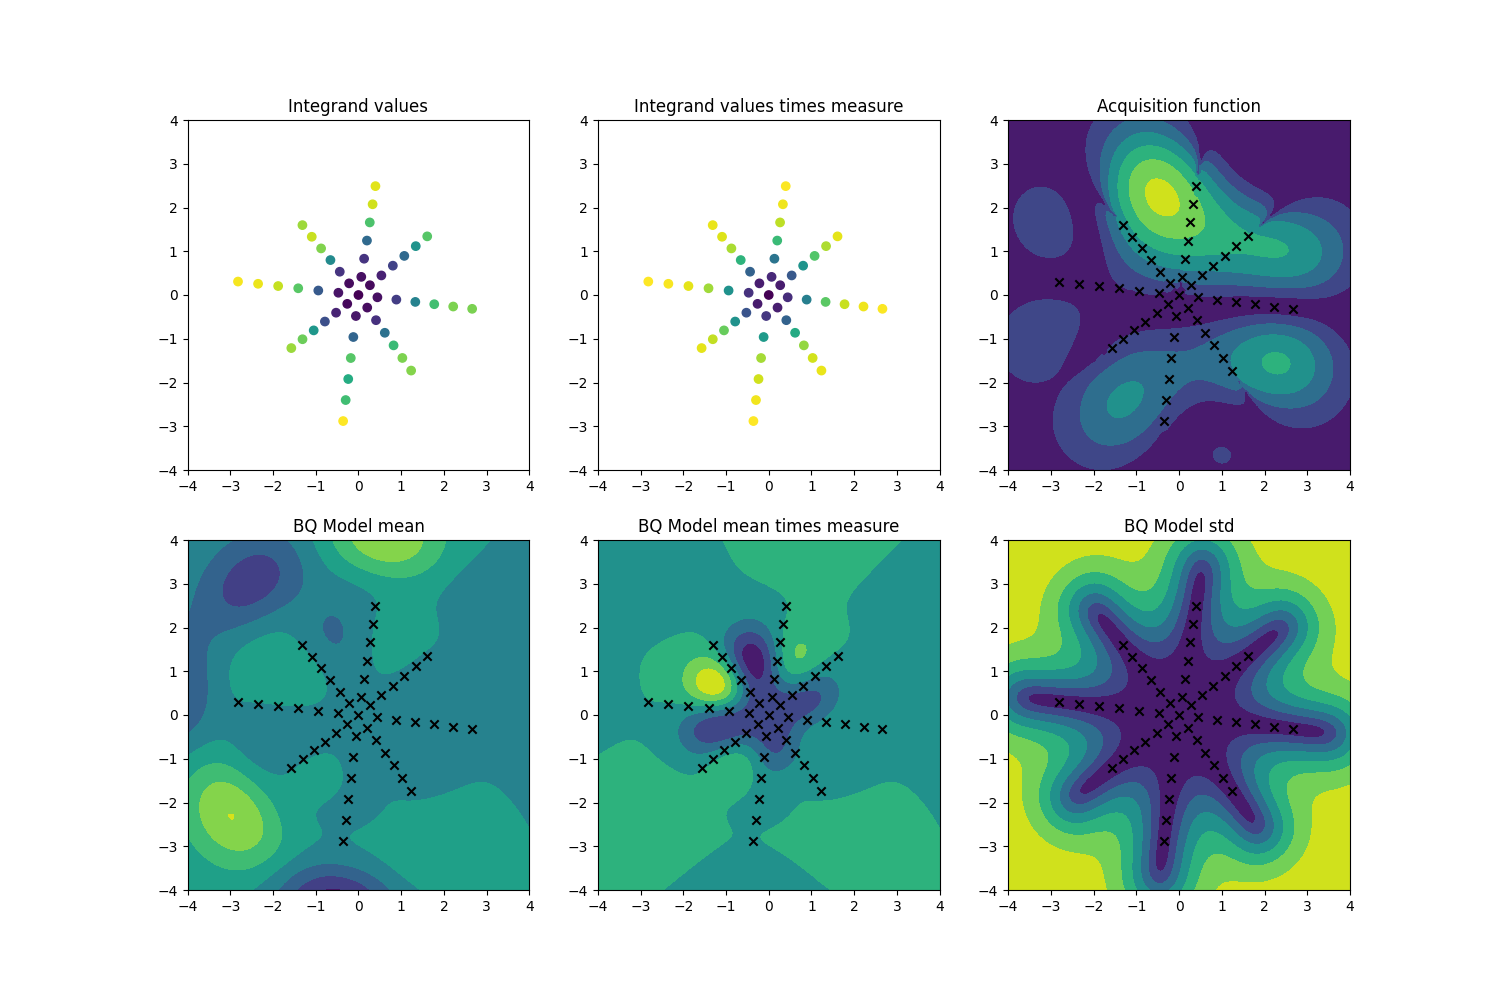
\includegraphics[width=1\linewidth]{report/figures/UFA_BQ_integrand_2d.png}
    \caption{Bayesian Quadrature. All figures represents model evaluations in one data point, and are seen from the space of the $v$-vector. Clockwise from upper left: The integrand values are the model evaluations, given the rays of the $v$'s. Here, 9 different values of $v$ has been explored and their corresponding ray traces can be seen. The second panel show the model evaluations multiplied by the integration measure - which is a standard normal normal distribution. The acquisition function in the third panel returns the expected variance reduction in the integral of the Gaussian Process, given that we evaluate our model in the specific point. The fourth panel shows the expected value of the underlying GP, whereas the fifth shows the underlying GP multiplied by the integration measure. The last panel shows the variance of the expected value of the underlying GP}
    \label{fig:UFA_BQ_integrand_vals_2d}
\end{figure}

As noted before, the Vanilla Laplace model allows for subspace sampling. This property is inherited in the other models. The idea extends to the Riemannian LA where the samples will lie close to the sub-manifold of the original loss manifold, extended by the most important eigenvectors from the Laplace approximation. In the case with a 1-dimensional sub-manifold within a 2-d loss manifold, we see that the samples lie on the same path that tends to lie close to the ridge induced by the most important eigenvector. See figure \ref{fig:banana_Riemann_1d_subspace_samples} for an intuition of the idea.
